\chapter{Ensamblaje e instrumentacion}

En este capitulo se presentaran todos los detalles del ensamblado del reflector parabolico, la instalacion del rotor y la integracion de estos con el soporte de la montura en el pedestal construido para el telescopio. Tambien se detallaran todos los instrumentos evaluados y seleccionados para la construccion del receptor de radiofrecuencia, el rack de control y la infraestructura de caracterizacion.\\

Junto con esto, se mosntraran todas las piezas diseñadas e impresas en 3D para el soporte del alimentador y todos los soportes especificos que se necesitaron para la instalacion de los distintos componentes del telescopio.\\

Para finalizar con la descripcion del software creado para la operacion, mantenimiento y caracterizacion del telescopio.\\

\section{Ensamblado Mecánico}

Tanto el reflector parabolico como la montura alt azimutal y su correspondiente controlador, son elementos adquiridos de la compañia \textit{RFHamdesign}, una empresa holandesa que se especializa en la construccion de telescopios de radio aficionados. El reflector de 3 metros venia completamente desarmado y con piezas que requerian ser modificadas y ensambladas para su correcto funcionamiento.\\

Para todo el ensamblado se utilizaron herramientas de y electricas, como taladors, tijeras de ojalata, remachadoras, etc.\\

\begin{figure}
    \centering
    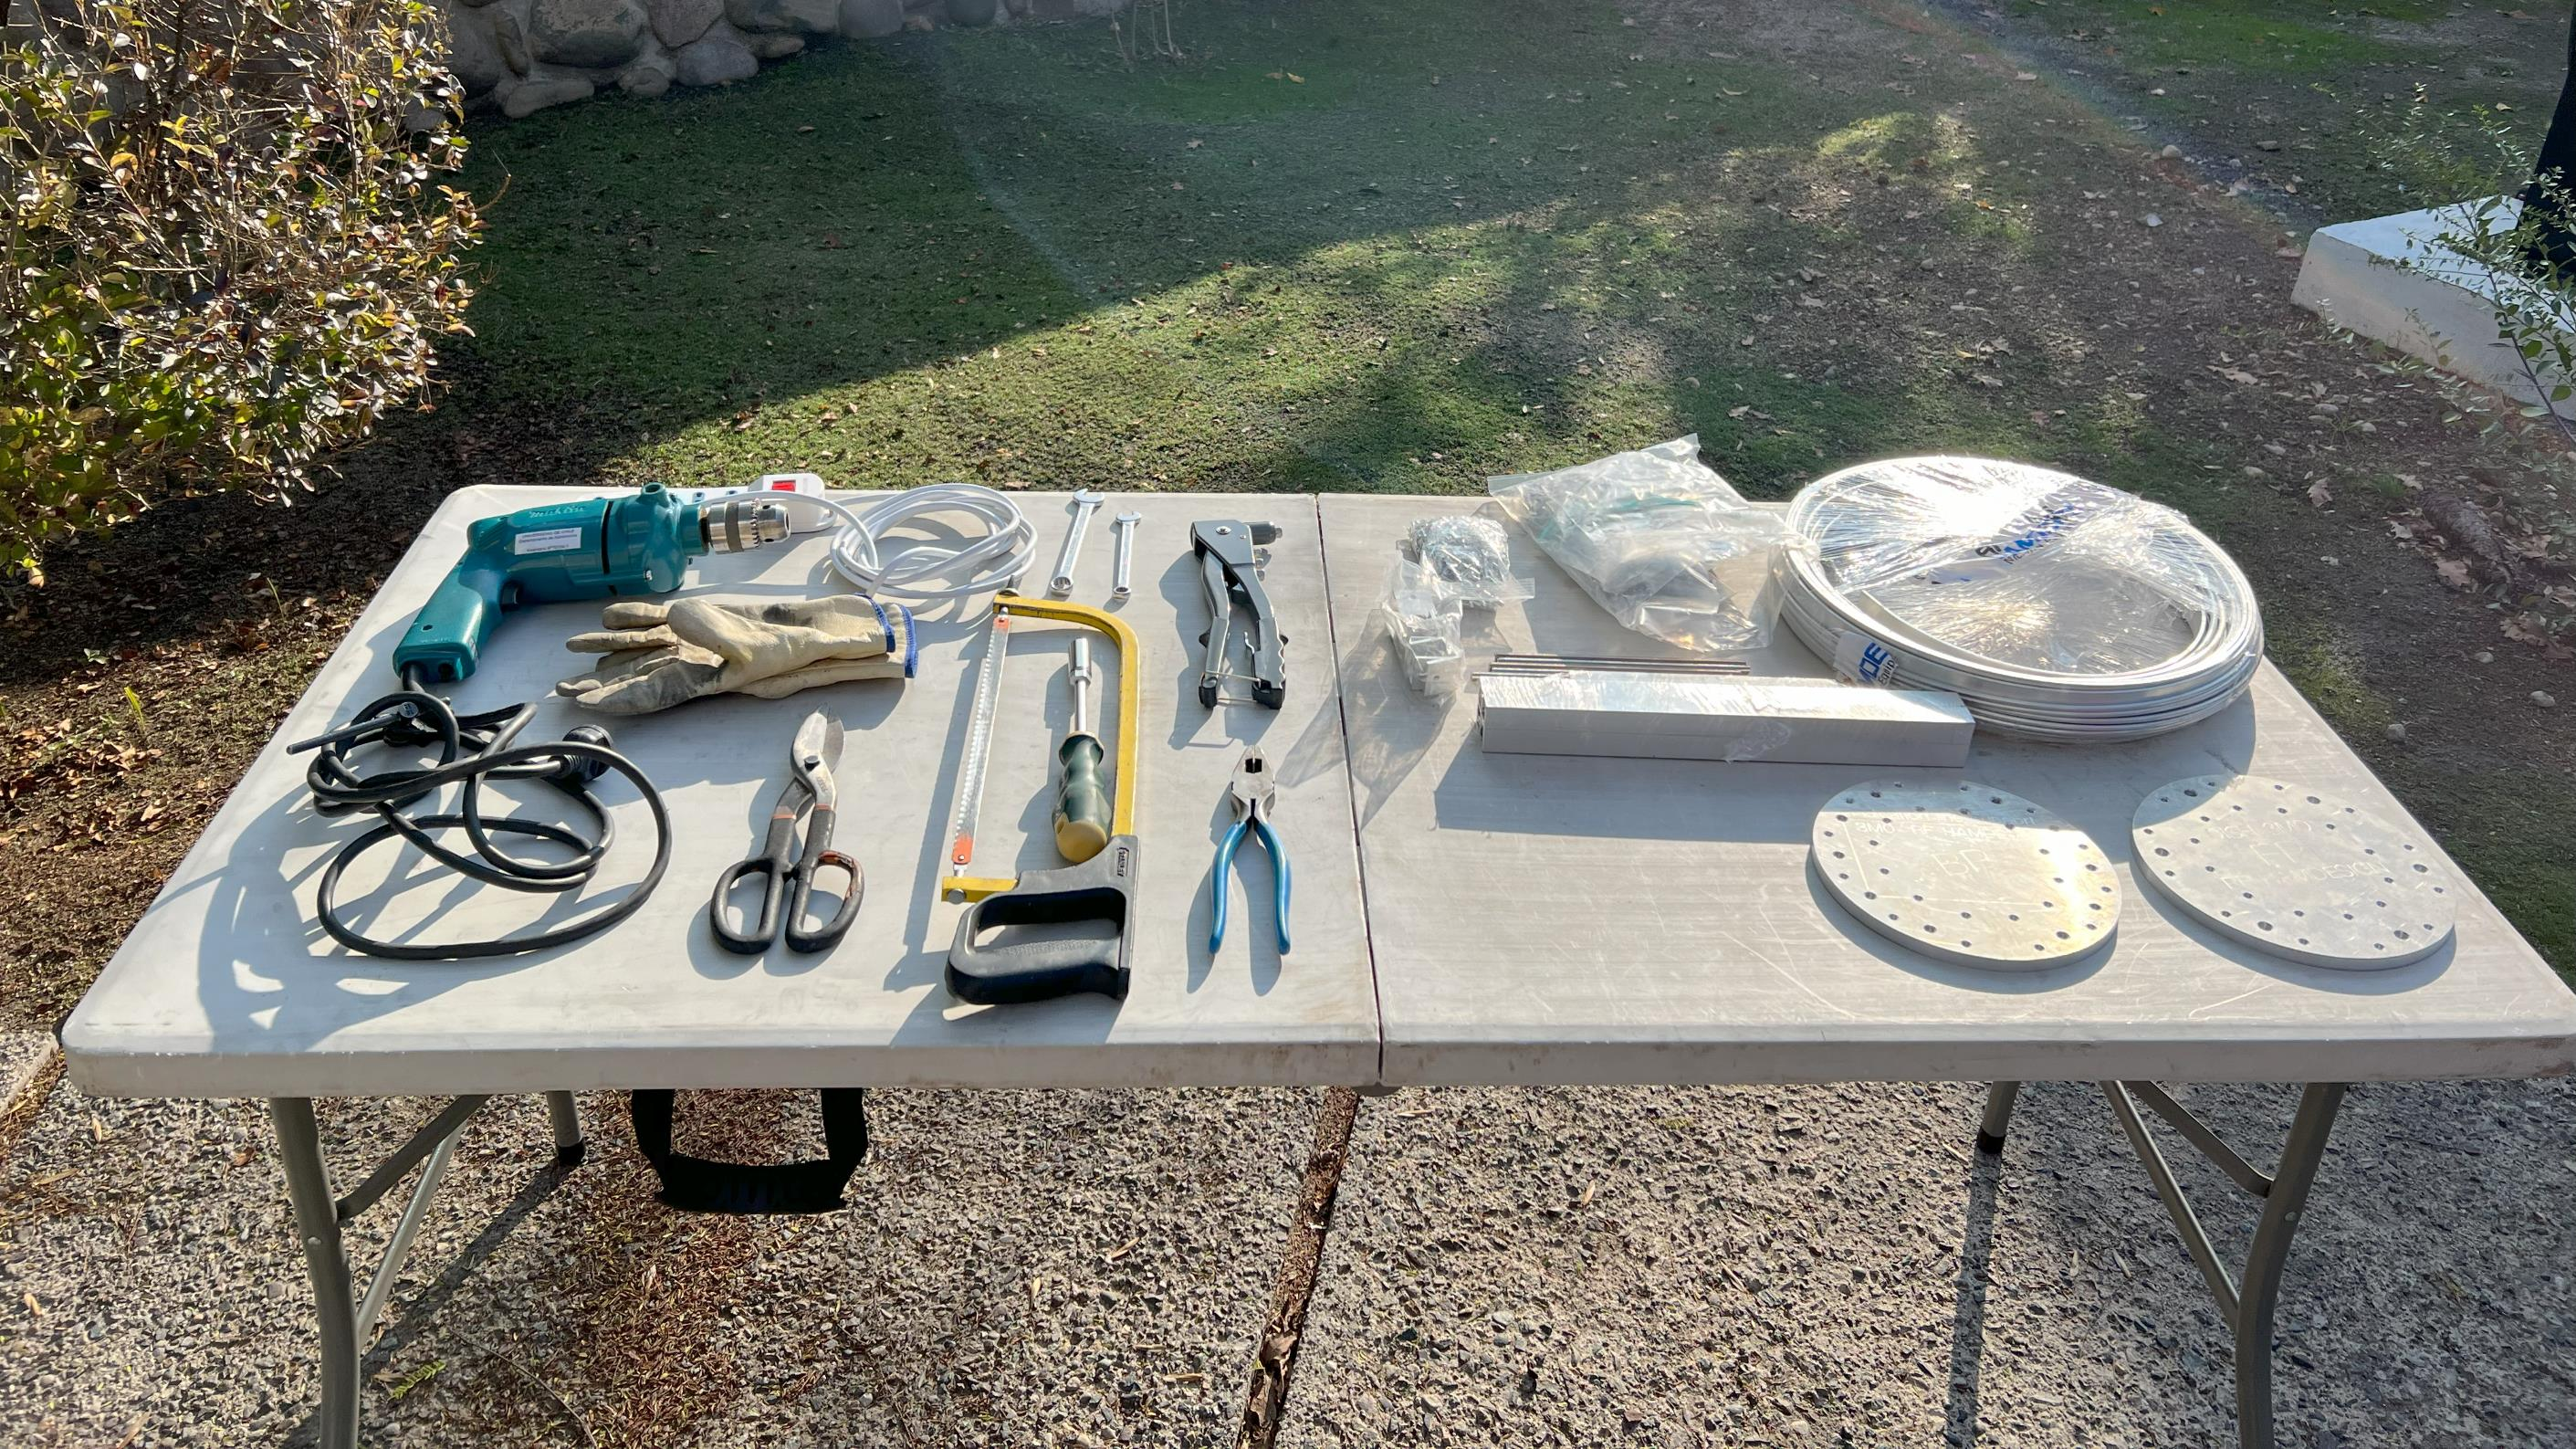
\includegraphics[width=0.8\textwidth]{img/herramientas}
    \caption{Herramientas utilizadas para el ensamblado de la superficie del reflector parabólico.}
    \label{fig:ensamblado1}
\end{figure}

En la figura \ref{fig:ensamblado1} se pueden ver las herramientas utilizadas para el ensamblado de la superficie del reflector parabólico ademas de las piezas que requerian de modificacion adicional para la instalacion correcta.\\

\subsection{Reflector Parabólico}

Las piezas del reflector se dividen en los 12 arcos, o costillas, de aluminio que conforman la estructura que da forma a la superficie parabolica, con un centro de aluminion donde estas 12 piezas se unen y apernan.\\

\begin{figure}
    \centering
    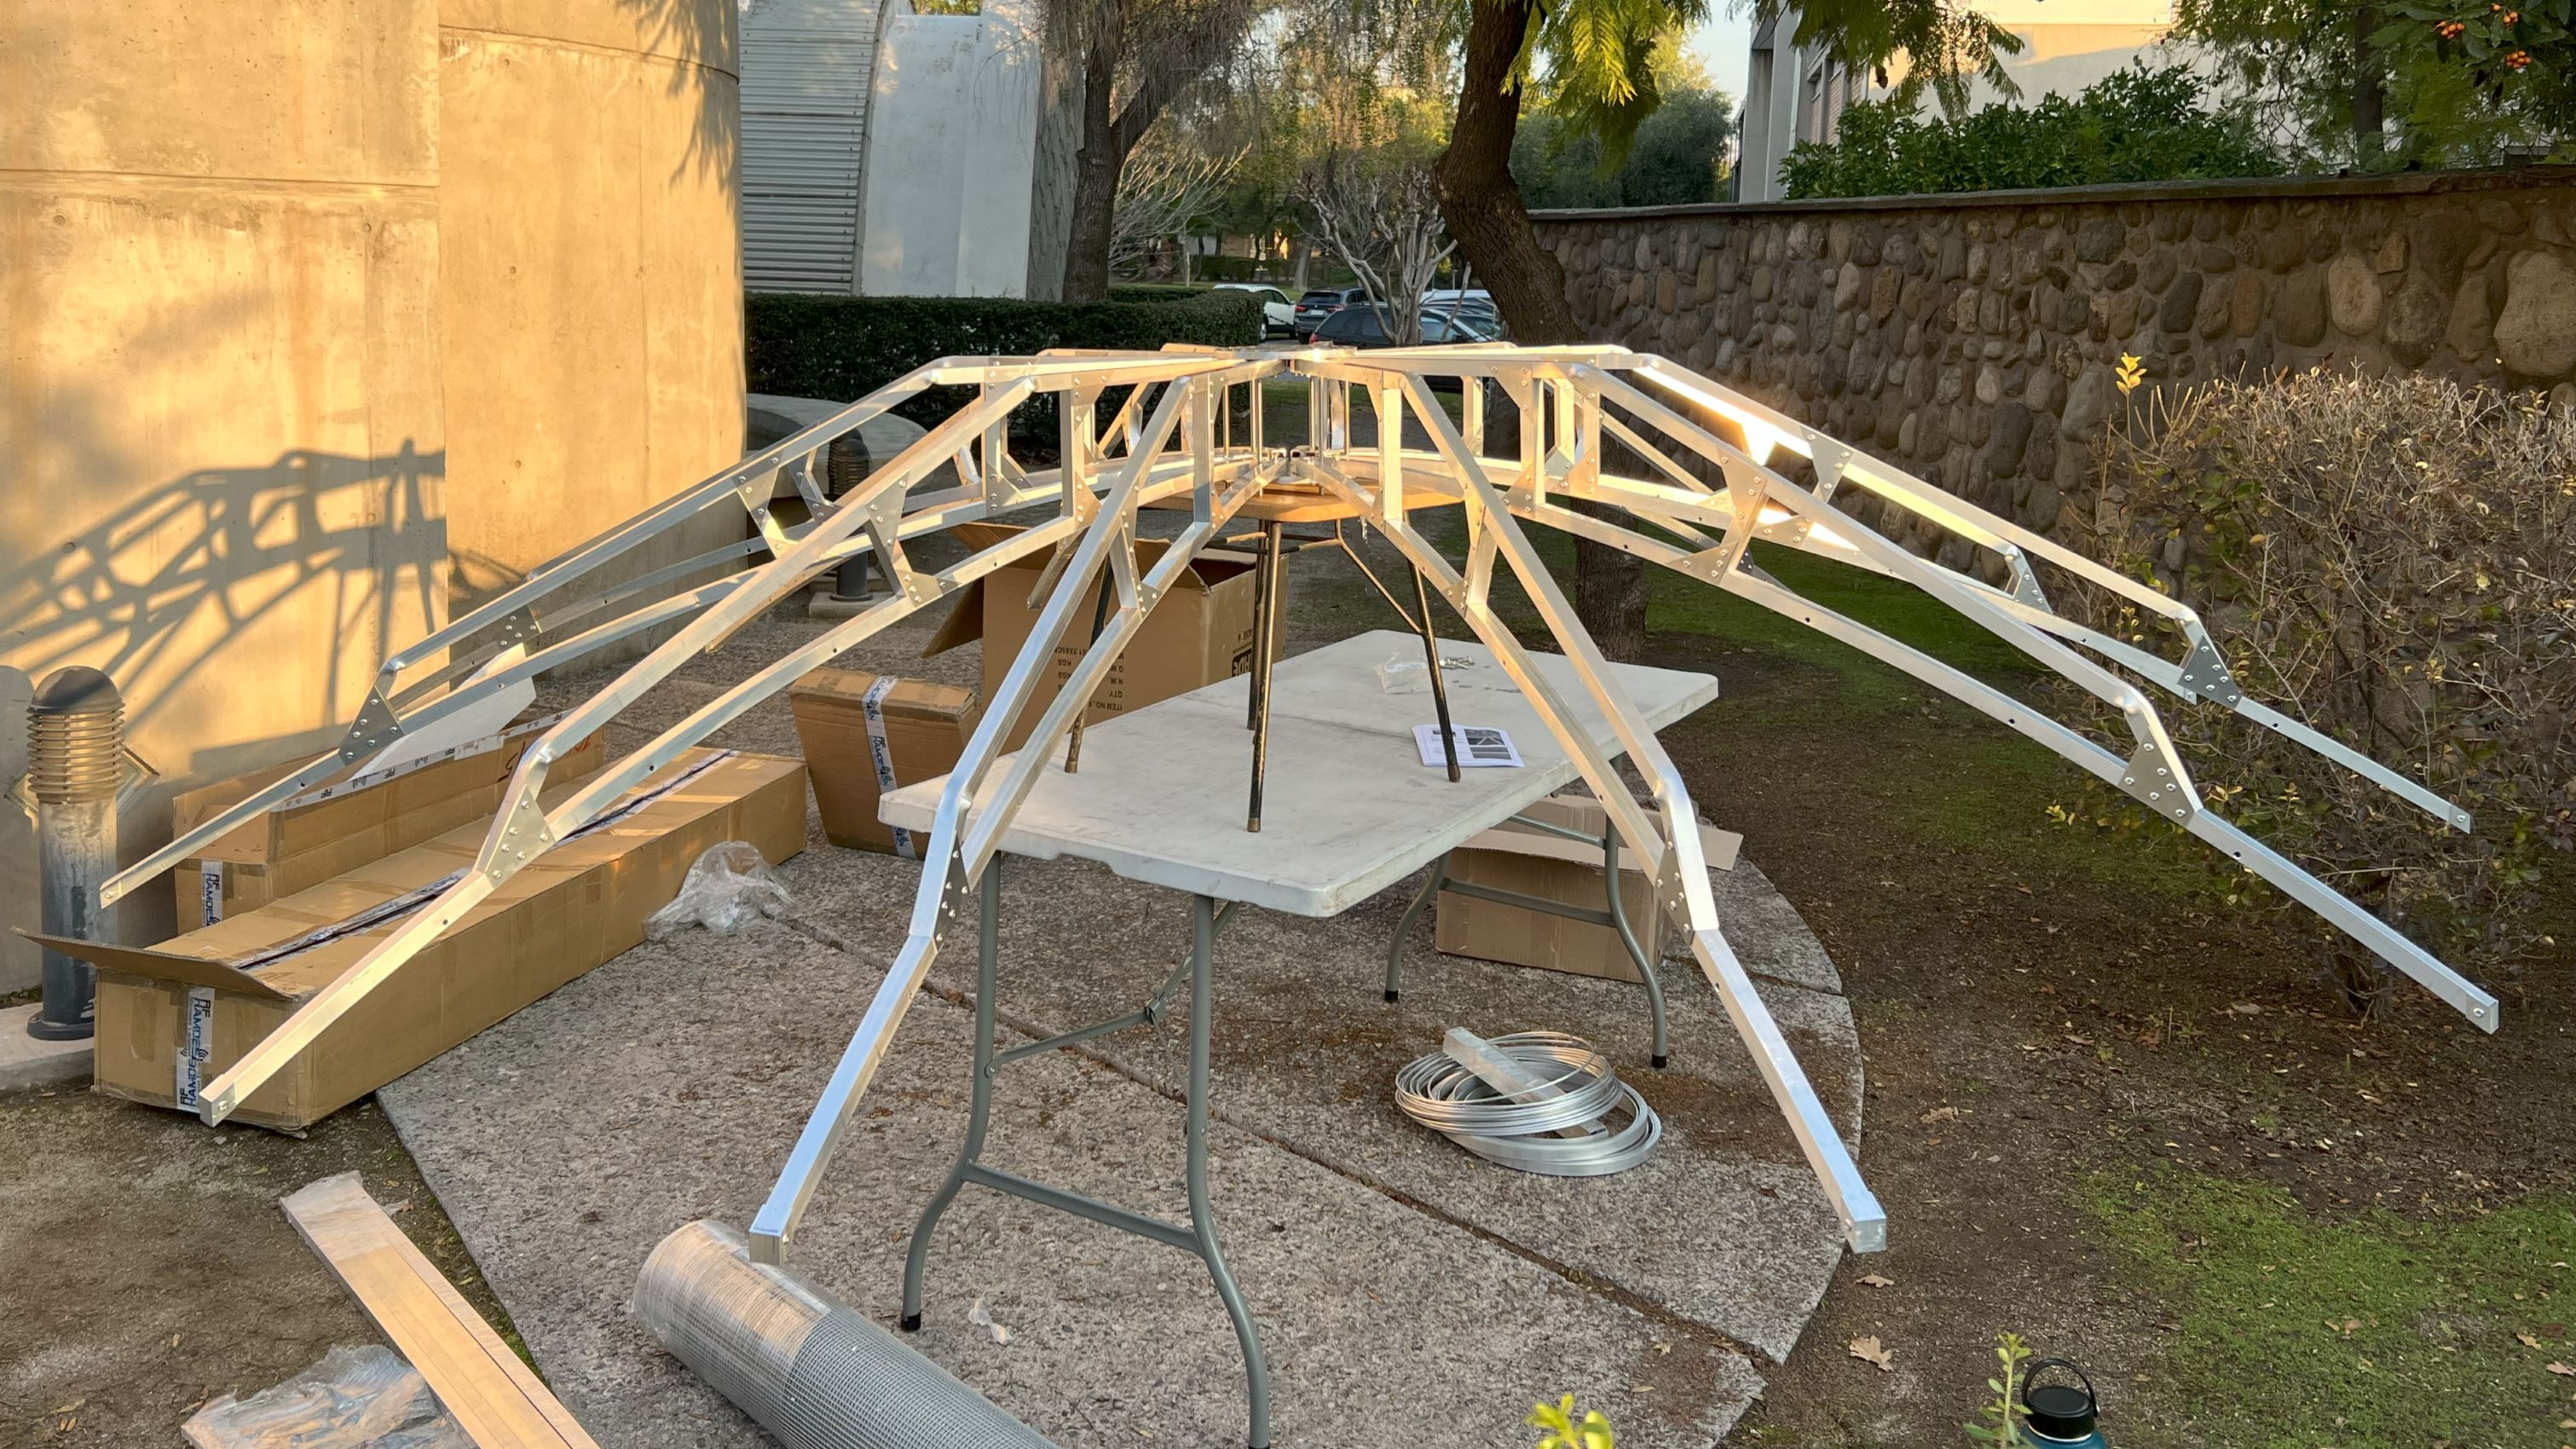
\includegraphics[width=0.8\textwidth]{img/estructura1}
    \caption{Los 12 arcos de alumunio apernados al centro del reflector parabólico.}
    \label{fig:ensamble2}
\end{figure}

En la figura \ref{fig:ensamble2} se pueden ver los 12 arcos de aluminio apernados a los discos de distribucion, que ademas es el punto de anclaje para el soporte de la montura.\\

Luego desenrollan y enderezan los tubos de aluminio que confirmar los anillos donde se tensaeran las mallas metalicas que conforman la superficie del reflector. Con la misma logica se toma la cinta de alumninio, que es aproximadamente de 4 mm de espesor, para enderesarla y prepara las perforaciones para los primeros remaches.\\

\begin{figure}
    \centering
    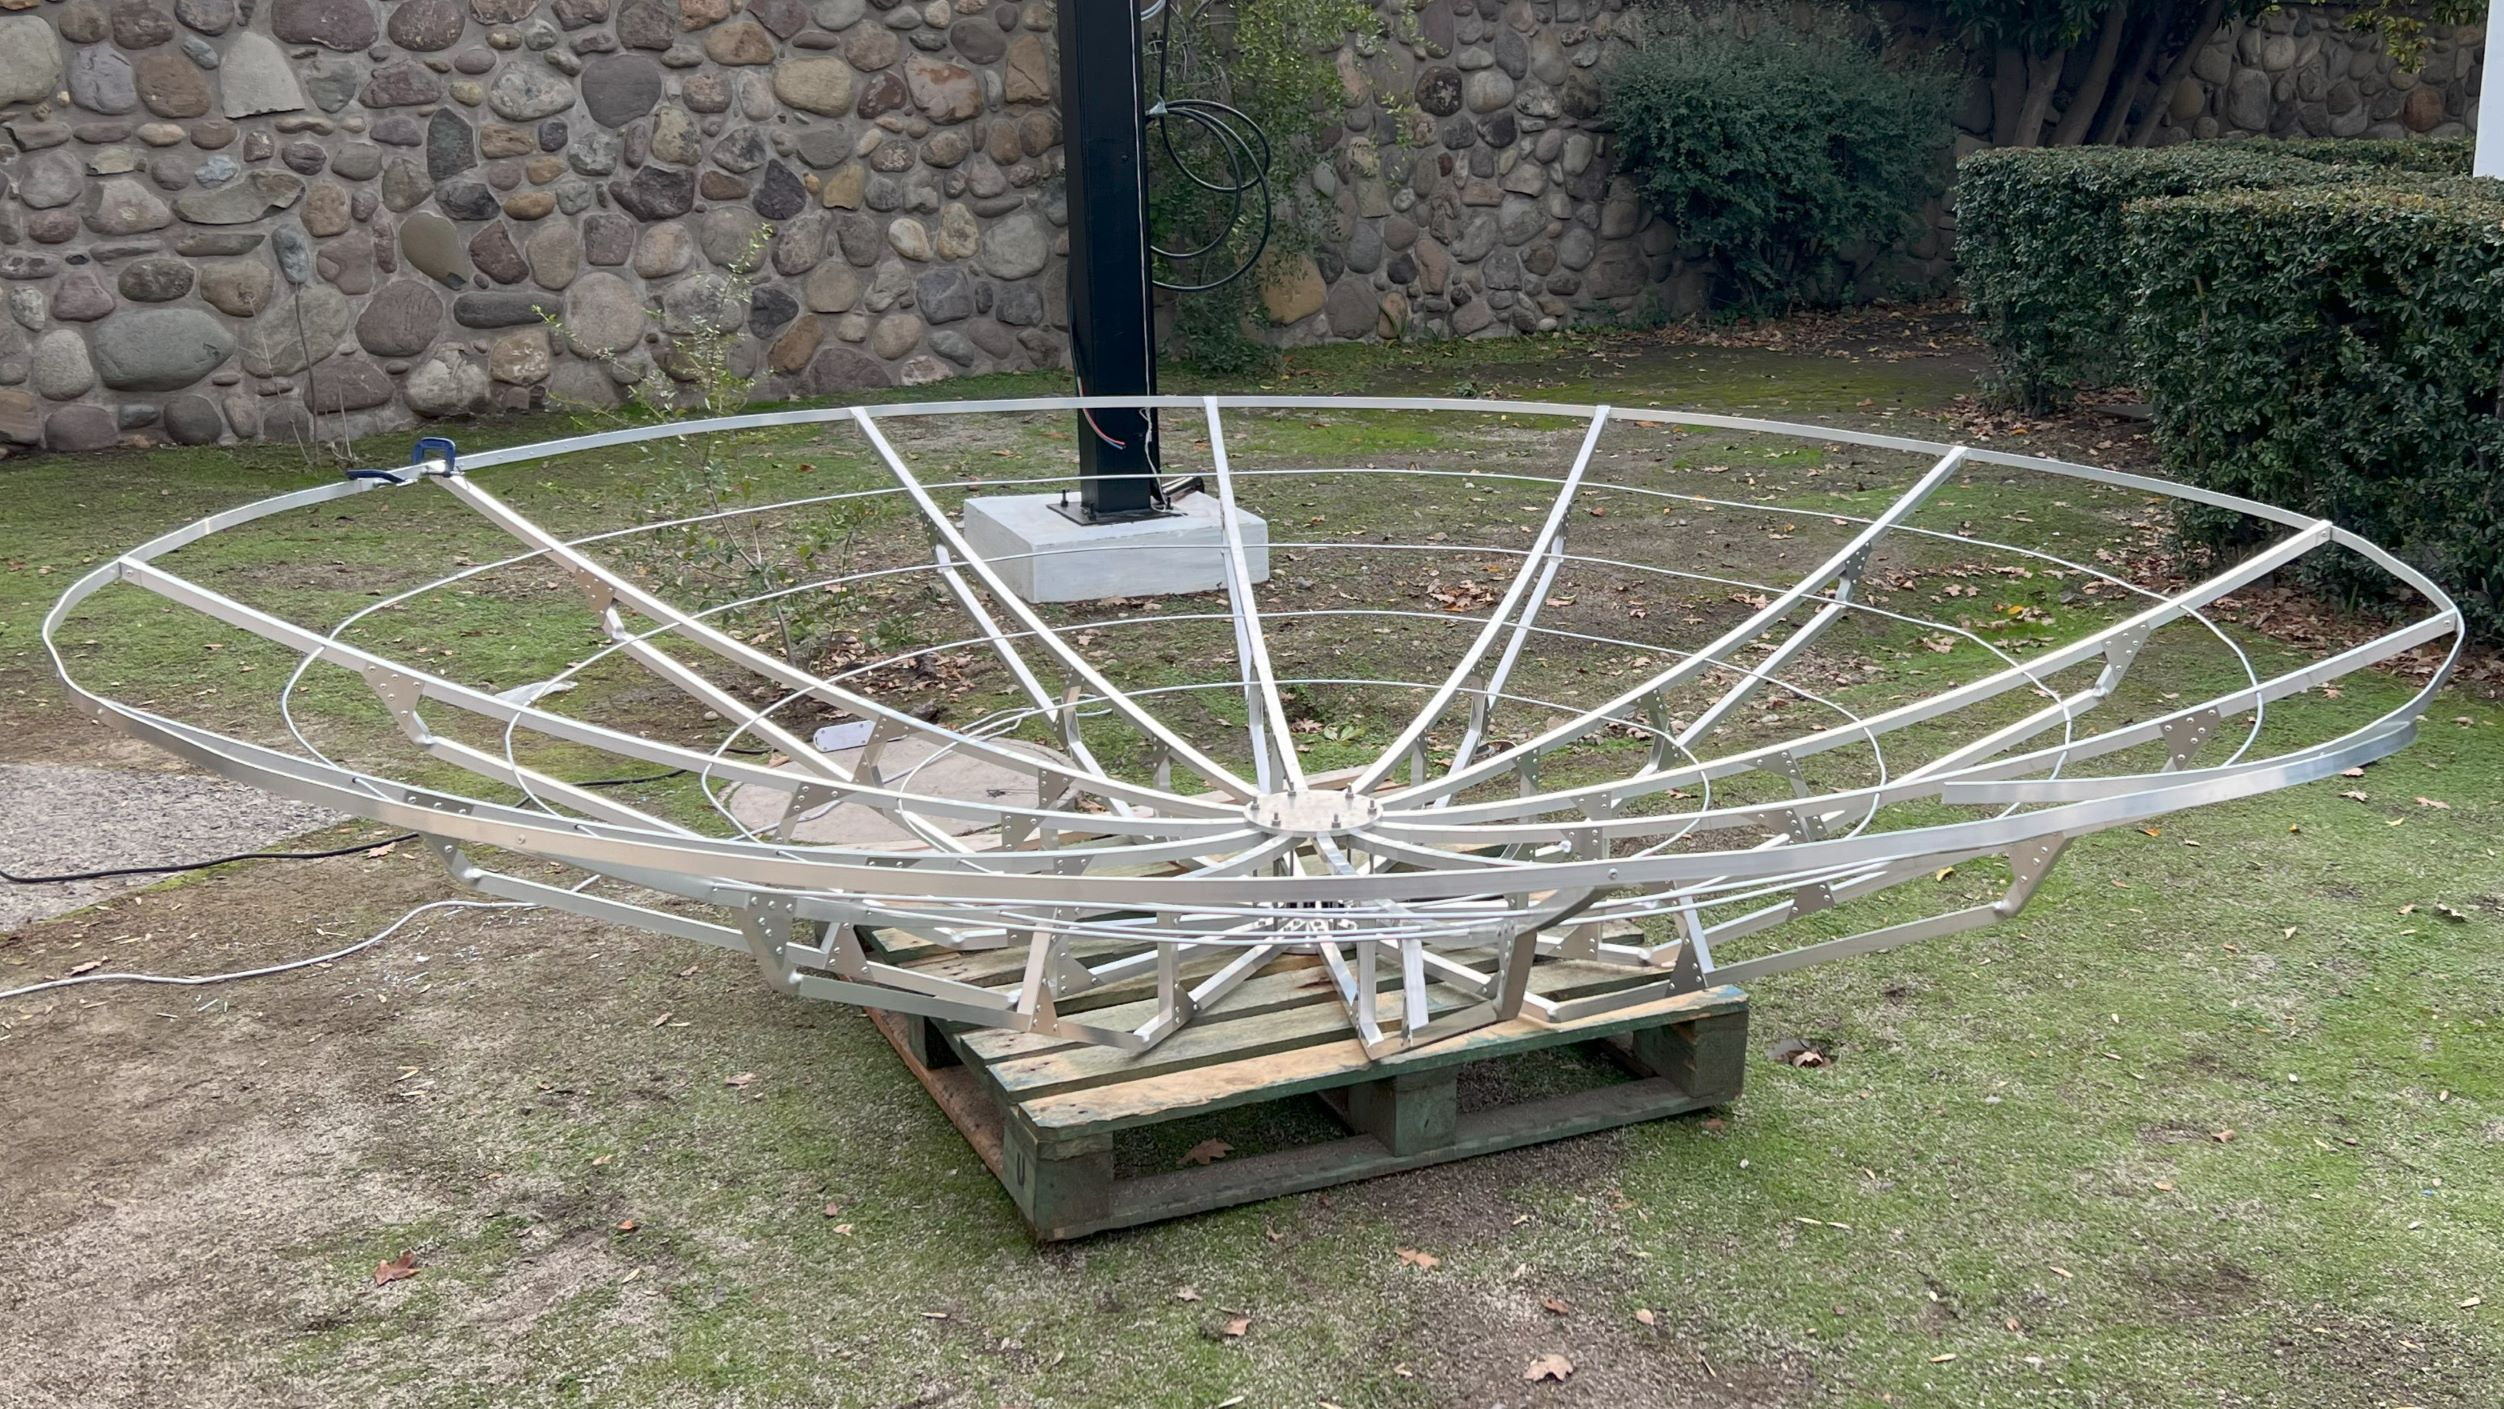
\includegraphics[width=0.8\textwidth]{img/estructura2}
    \caption{Los tubos de aluminio y la cinta de aluminio para la tensión de la malla metálica instalados radialmente en los soportes.}
    \label{fig:ensamble3}
\end{figure}



\subsection{Diseño de soportes adicionales}

\subsection{Montura Alt-Azimutal}

\subsection{Rack de control}

\section{Alimentador}

\section{Diseño del receptor}

\subsection{Cadena de recepción}

\subsection{Digitalizador y adquisición}

\section{Software de control y adquisición}

\subsection{Control de la montura}

\subsection{Adquisición de datos}

\section{Infraestructura de caracterizacion}

\subsection{Fuente de calibración}

\subsection{Fuente de ruido}

\subsection{Software de caracterización}